
We implemented $\THESYSTEM$ as a tool which takes a labeled program as input
and outputs the upper bound on the program adaptivity and the total number of queries that the program runs.
This implementation consists of a module written in OCaml for the generation of the estimated graph $\progG$, and a module written in Python for the weight estimation algorithm (Section~\ref{sec:alg_weightgen}) and the algorithm $\pathsearch$ (Section~\ref{sec:alg_adaptcompute}).
The OCaml program takes the labeled program as input and outputs a version of the graph $\progG$ (without weights) and the abstract transition graph $\absG$ for the program. These two objects are then
fed into the python program which computes the weights, and outputs the adaptivity bound and the query number.
%
We evaluated this implementation on $25$ examples with performances summarized in Tab.~\ref{tb:adapt-imp}.
The $1^{st}$ column is the example name.
For each example $c$, the $2^{nd}$ column is its adaptivity rounds,
$\THESYSTEM$ outputs are in the the $3^{rd}$ and $4^{th}$ columns. They are
% two expressions.
% The first one is 
the adaptivity upper bound and
% the second one is the 
% upper bound for
$c$'s total query requests \#. 
The last $4$ columns are {\THESYSTEM}'s performance w.r.t. the program lines.
We track the running time of the OCaml code for parsing the program and generating the $\progG(c)$,
and the running times of the weight analysis
and the $\pathsearch(c)$ in Python.
We implemented two weight estimation methods. The first one (referred as I in Tab.\ref{tb:adapt-imp}) is the one we presented formally in Section~\ref{sec:alg_weightedgegen}. Unfortunately, this method is accurate but slow, it doesn't performs well with big program. The second one (referred as II) is a relaxation of the first one. It is more  efficient but it over-approximate complicated loops. Based on the two implementations, our $\THESYSTEM$ produces two bounds on the adaptivity, corresponding to the left and right side (I | II) in the $3^{rd}$, $4^{th}$ and $6^{th}$ columns\footnote{When the method II produces the same results as I, we omit them and use the symbol $-$.}.
%
The first $5$ programs are adapted from classical data analysis algorithms.
$\THESYSTEM$ computes tight adaptivity bound for the first 3.
For the forth program $\kw{multiRoundsO(k)}$, $\THESYSTEM$ over-approximates the adaptivity as $1 + 2*k$ because of its path-insensitivity.
The fifth program is the one in Example~\ref{ex:multiRoundsS}, where $\THESYSTEM$ outputs the tight bound but we give a loose definition for its actual adaptivity.
%
% The first two examples $\kw{twoRounds(k)}$, $ \kw{multiRounds(k)}$ are the same as Figure~\ref{fig:overview-example}(a) and Figure~\ref{fig:multipleRounds}(a).
The programs from Tab.~\ref{tb:adapt-imp} line:6-17 all have small size but complex structures, to test the programs under different situations including
data, control dependency,
the multiple paths nested loop with related counters, etc.
Both implementations compute tight bounds for examples in line:6-14
and over-approximate the adaptivities for $15^{th}$ and $16^{th}$ due to path-insensitivity.
For the $17^{th}$ one, implementation I gives tight bound bound while II gives loose bound, so we keep both implementations.
The last six programs are big but simple,
to test the performance limitation. 
From the evaluation results, the performance bottleneck is the weight estimation algorithm.
The implementation I
% By implementing the bound analysis algorithm in Section~\ref{sec:alg_weightgen} (adapted from \cite{sinn2017complexity}), we are 
is unable to evaluate them in a reasonable time period, denoted by $*$ on the left side.
While the implementation II computes the \emph{adaptivity} for
them effectively on the right side. 
% Overall for these examples, our system gives both the accurate adaptivity definition and estimated
% adaptivity upper bound through our formalization and analysis framework $\THESYSTEM$.
% The complete programs can be found in the Appendix.

{\footnotesize
\begin {table}[H]
\vspace{-0.4cm}
    \caption{Experimental results of {\THESYSTEM} implementation}
    \vspace{-0.5cm}
        \label{tb:adapt-imp}
        \begin{center}
        \centering
{\tiny
        \begin{tabular}{| >{\tiny}r | c | c | c | c | c | c | c | c | c | c | c }
         \hline \hline
        \multirow{2}{*}{Program $c$} & 
        \multirow{2}{*}{\emph{adaptivity}}
         & \multicolumn{2}{c|}{$\THESYSTEM$}
         & {L.O.C}
         & \multicolumn{3}{c|}{running time (second)} \\ 
         \cline{3-8}
         & & {$\pathsearch(c)$ } & {$\query$\# } &  & graph & weight & walk \\ 
         \cline{6-8}
        %  & & & &  & $\THESYSTEM$-I & $\THESYSTEM$-II & $\THESYSTEM$-III  \\
         \hline \hline
         $  \kw{twoRound(k)}$ & $2$ &  $2| -$ & $k+1 | -$  & 8 & 0.0005 & 0.0017 | 0.0002 & 0.0003 \\
         $  \kw{mR(k)}$ & $k$ &  $k| \max(1,k)$ & $k| -$  &  10 & 0.0012 & 0.0017 | 0.0002 & 0.0002 \\
         $  \kw{lRGD(k, r)}$ & $k$ & $k | \max(1,k) $ & $ 2k | -$  &  10 & 0.0015 & 0.0072 | 0.0002 & 0.0002  \\
         $  \kw{mROdd(k)}$ & $1 + k$ &  $2+\max(1,2k) | - $ & $1 + 3 k | - $  &  10 & 0.0015 & 0.0061 | 0.0002 & 0.0002 \\
         $  \kw{mRSingle(k)}$    & $2$ &  $1+ \max(1, k) | -$ & $1 + k | 1 + k$  &  9 & 0.0011 & 0.0075 | 0.0002 & 0.0002 \\
        %  $  \kw{seq()}$ & $4$ & $4$ & $4$ & 4 & 0.0016 & 0.0002 & 0.0001 \\ 
        %  $  \kw{seqRV()}$ & $4$ & $4$ &  $4$ & 4 & 0.0011 & 0.0003 & 0.0001 \\  
        %  $  \kw{ifVD()}$ & $3$ & $3$ &  $3$ & 5 & 0.0010 & 0.0005  & 0.0001 \\
         $  \kw{ifCD()}$ & $3$ & $3 | 4$ &   $3| 4$  & 5 & 0.0005 & 0.0003 | 0.0001  & 0.0001 \\
         $  \kw{loop(k)}$ & $1+k/2$ &   $1 +\max(1, k/2) |- $  &  $1+k/2 | - $ & 7 & 0.0021 & 0.0015| 0.0001 &  0.0001 \\
         $  \kw{loopRV(k)}$ & $1 + 2k$ &  $1 + 2k| 1 + \max(1,2k)$ & $2 + 3 k| -$  &  9 & 0.0016 & 0.0056| 0.0002 & 0.0001  \\
         $  {\kw{loopVCD(k)}} $ & ${1 + 2Q_m}$ &  ${Q_m+\max(1,2Q_m)}$ | - & $2+2Q_m$ | -  &  6 & 0.0016 & 0.0007 |0.0002 & 0.0001 \\
         $ {\kw{loopMPVCD(k)}}$ & $2+Q_m$ &  $2 + Q_m$ | - & $2+2Q_m$ | -  &   9 & 0.0017 & 0.0043 | 0.0002 & 0.0001 \\
         $  \kw{loop2VD(k)}$ & $2 + k^2$ &   $3 + k^2| -$ & $1 + k + k^2|- $   &  10 & 0.0018 & 0.0126 | 0.0002 & 0.0001  \\
         $  \kw{loop2RV(k)}$ & $1 + k +  k^2$ &  
         $ 2 + k +  k^2 | -$ 
         &  $2 + k + k^2| -$   &  10 & 0.0017 & 0.0186 | 0.0002 & 0.0001  \\
         $  \kw{loop2MV(k)}$ & $1 + 2k $ & $1 + \max(1,2k) | -$ &  $1 + k + k^2 |-$  & 10 & 0.0016 & 0.0071 | 0.0002 & 0.0001 \\
         $ \kw{loop2MPRV(k)}$ & $1 + k + k^2$ &  $3 + k + k^2  | -$ &  $2 + 2k + k^2 | - $  &  10 & 0.019 & 0.0999 | 0.0002 & 0.0002 \\
         {$ \kw{loopM(k)}$} & $1 + k$ &  $ 2 + \max(1,2k) | -$ & $1 + 3k | - $  &  9 & 0.0017 & 0.0062 | 0.0002 & 0.0001  \\
         {$ \kw{loopM2(k)}$} & $1 + k$ &  $ 2 + k | -$ & $1 + 3k | - $  &  9 & 0.0017 & 0.0062 | 0.0002 & 0.0001  \\
         {$\kw{loop2RC(k)}$} & $1 + 3k$ &  $1 + 3k | 2 + 3k + k^2$ &  $1 + 3k | 1 + k + k^2$  &  11 & 0.019 & 0.2669 | 0.0002 & 0.0007 \\
         $  \kw{mR(k, N)}$ & $k$ & $ k | -  $ & $k |-$   &  27 & 0.0026 & 85.9017 | 0.0003 & 0.0004 \\
         $  \kw{mRC(k)}$ & $2k$ & $  2k | -$ & $ 2k | -$   &  46 & 0.0036 & 5104 | 0.0003 &  0.0013\\
         $  \kw{seqC(k)}$ & $12$ & $12  $ | - & $326 | -$  &  502 & 0.0426  & 1.2743 | 0.0003 & 0.0223 \\
         $  \kw{tRC(k)}$ & $2$ &  $ * | 2$ & $* | 1 + 5k + 2 k^2 $  &  42 & 0.0026 & * | 0.0003 & 0.0005\\
         $  \kw{{jumbo(k)}}$ & $ \max(20, 8+k^2)$ &  $ * | \max(20, 6+k+k^2)$   &   $* | {44+k+k^2} $  &  71 & 0.0035 & *| 0.0003 &  0.0085 \\
        %  $  \kw{jumbo(k)}$ & $ \max(20, 10+k+k^2 )$ &   $* | \max(20, 12 + k+ k^2)$  &  $* |286+26k+10k^2$   &  502 & 0.0691 & * | 0.0009 & 0.018 \\
         $  {\kw{big(k)}} $ & $22+k+k*k$ &  $* |28 + k + k^2$ &  $* |121+11k+4k^2 $  &  214 & 0.0175 & * | 0.0004 & 0.002 \\
         \hline \hline
        \end{tabular}
}
\end{center}
\end{table}
}




On the tensorflow, sklearn and pytorch bechmarks. These programs are widespread in real-world machine learning area.

These programs include  
15 data analysis programs 
from \hyperlink{https://github.com/scikit-learn/scikit-learn/tree/main/examples}{sklearn}~\cite{SklearnBenchmark} benchmark,
21 machine learning programs
from \hyperlink{https://github.com/tensorflow/tensorflow/tree/master/tensorflow/examples}{tensorflow}~\cite{TensorflowBenchmark} 
and \hyperlink{https://github.com/pytorch/pytorch}{pytorch}~\cite{PytorchBenchmark}
benchmarks,
and 4 programs implementing the strategies from~\cite{Jamieson2015TheAO}.
% \hyperlink{https://homes.cs.washington.edu/~jamieson/resources/kevinJamieson\_Dissertation.pdf}{thesis}.

The 15 data analysis programs 
from sklearn benchmark includes 12 programs with 2-adaptivity rounds
and 3 programs with 4-adapvitiy rounds.
% for the database classification.
These 2-rounds adaptivity programs are
the
implementation of the decision tree, logistic regression, naive Bayesian inference models equipped with non-adaptive optimizer, grid search.
The 4-rounds adaptivity programs are
the implementation of the same models equipped with one v.s. rest model
and k-means model and the grid search optimizer as well.
These programs are evaluated for classifying a demography dataset from 
the USA census database~\cite{CensusDatabase}.

For each program, we plot its generalization error measured by root mean square error over fresh testing data.
Then with our tool, we choose different mechanism and evaluate each over the same data.
The result shows that for the same data analysis program, the generalization error is reduced
by equipping with the proper mechanism chosen by our model.

The 21 machine learning programs
from \hyperlink{https://github.com/tensorflow/tensorflow/tree/master/tensorflow/examples}{tensorflow}
and \hyperlink{https://github.com/pytorch/pytorch}{pytorch}
benchmarks include
3 fully-adaptive progress data analysis
strategy~\cite{ZrnicH19}.
Specifically they are the implementation of the recurrent neural network, long short term models for 
weather forecasting.

9
fully-adaptive conservative data analysis
strategy~\cite{ZrnicH19}.
Specifically they are the implementation of the convolutional neural network, transfer learning model,
and multiple-dense layer neural networks equipped with gradient decedent optimizer for
weather forecasting, image classification over MNIST dataset
% through fitting the  CNN, RNN, LSTM models for image classification and 
% weather forecasting as well.

9 programs with two adaptivity rounds for text classification,
article classification, action recognition over real world databases.


Implemented~\cite{Jamieson2015TheAO}.

We translate these programs into our syntax.
For comparison, we also report the results of 
four alternative versions of our \THESYSTEM.

{\small
\begin{figure}
\centering
\begin{subfigure}{.322\textwidth}
\begin{centering}
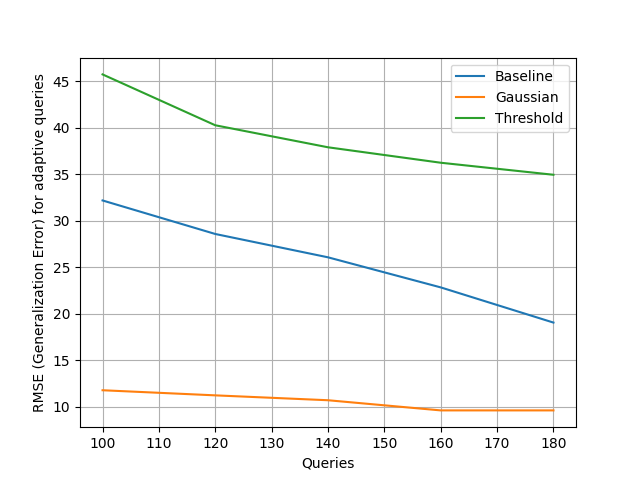
\includegraphics[width=1.0\textwidth]{cnn.png}
\caption{}
\end{centering}
\end{subfigure}
\quad
\begin{subfigure}{.322\textwidth}
\begin{centering}
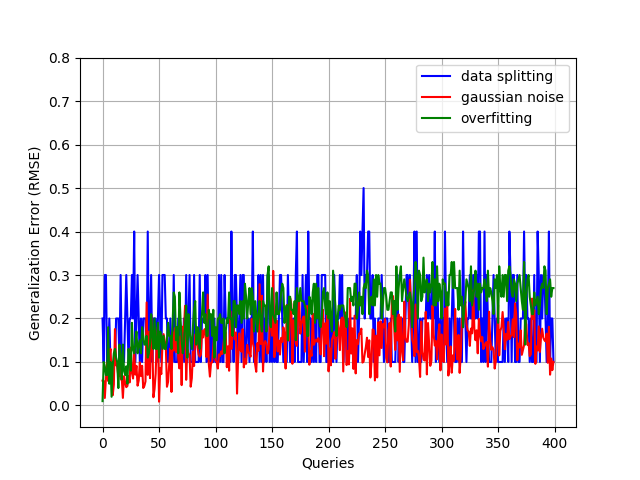
\includegraphics[width=1.0\textwidth]{multipleround.png}
\caption{}
\end{centering}
\end{subfigure}
\begin{subfigure}{.322\textwidth}
\begin{centering}
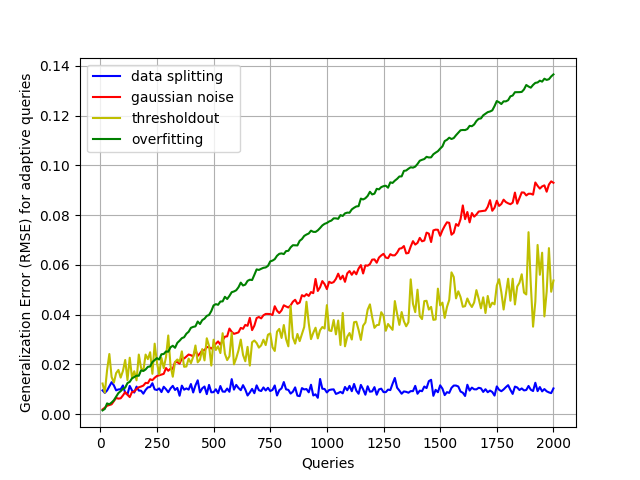
\includegraphics[width=1.0\textwidth]{twoRounds-rmse-fourmechs.png}
\caption{}
\end{centering}
\end{subfigure}
\vspace{-0.2cm}
 \caption{
 (a) The fully adaptive programs, 
 (b) The programs with constant number of adaptivity.
 (c) The programs implementing~\cite{Jamieson2015TheAO}
}
\label{fig:implementation_generalization_errors}
\vspace{-0.6cm}
\end{figure}
}
